\documentclass[tikz,border=14pt]{standalone}
\usepackage{amsmath,amssymb}
\usetikzlibrary{arrows.meta}
\definecolor{ink}{HTML}{E4EDF8}
\definecolor{muted}{HTML}{596B80}
\definecolor{blue}{HTML}{9FC2FF}
\definecolor{teal}{HTML}{63D3BB}
\definecolor{gold}{HTML}{E7C274}
\definecolor{panel}{HTML}{111923}
\pagecolor{panel}
\color{ink}
\begin{document}
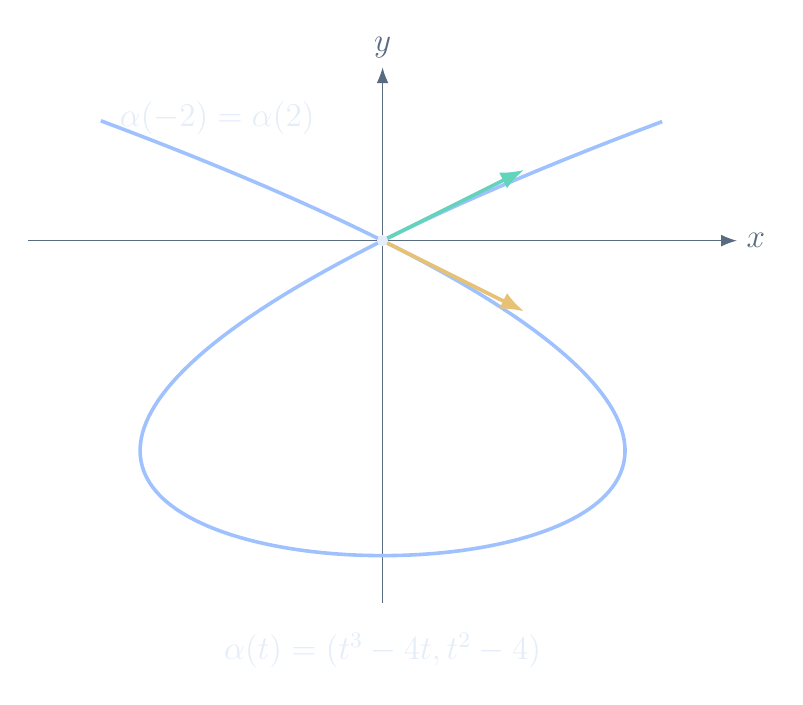
\begin{tikzpicture}[font=\large,text=ink,vec/.style={-{Latex[length=3mm]},line width=1.3pt},axis/.style={muted,-{Latex[length=2mm]},thin}]

\draw[axis] (-4.5,0)--(4.5,0) node[right] {$x$};\draw[axis] (0,-4.6)--(0,2.2) node[above] {$y$};
\draw[blue,line width=1.3pt] plot[domain=-2.35:2.35,samples=180] ({\x*\x*\x-4*\x},{\x*\x-4});
\draw[vec,teal] (0,0)--(1.8,.9);\draw[vec,gold] (0,0)--(1.8,-.9);
\fill[ink] (0,0) circle(2pt);\node at (-2.1,1.55) {$\alpha(-2)=\alpha(2)$};
\node[text=ink] at (0,-5.2) {$\alpha(t)=(t^3-4t,t^2-4)$};

\end{tikzpicture}
\end{document}
